\documentclass[cnatzke_thesis_proposal.tex]{subfiles}
\begin{document}

\chapter{Application to RIB : Mass 72 $\beta^-$ Decay}

With the demonstration that GRIFFIN can observe nuclear two-photon decays via a source measurement, the same analysis and event selection techniques can be applied to a short-lived isotope delivered by radioactive ion beams. 
Two $\beta$-decay experiments have been performed at TRIUMF, in 2017 and 2018, where a high-intensity radioactive beam of various gallium masses was delivered to GRIFFIN. 
\ref{tab:ga_beam_parameters} details the amount of data collected in hours and the average beam intensity during implantation.
The data analysis framework developed in the proof-of-concept testing (Section~\ref{sec:proof_of_concept_90sr}) will be applied to a radiactive beam dataset that has already been rigorously analyzed for investigations in the different configurations of even-even germanium isotopes.
Gallium masses 72, 74, 76, and 78 were delivered to the GRIFFIN decay station and ultra-high-statistics datasets, the beam was $\approx 10^{4-6}$ particles per second, were collected and rigorously analyzed by C. Porzio for her doctoral dissertation~\cite{porzio_configuration_2021}.
Of the four isotopes of delivered to GRIFFIN gallium-72 ($^{72}$Ga) provides an opportunity to make the first observation of two-photon decay in germanium-72 ($^{72}$Ge) and would only be the fourth observation of non-competitive two-photon decay in an isotope; the previous three isotopes are $^{16}$O, $^{40}$Ca, and $^{90}$Zr.

\begin{table}[]
  \centering
  \begin{tabular}{cccccc}
                                                                 & Beam      & Ion Source & Tape Cycle   & \begin{tabular}[c]{@{}c@{}}Hours of Data \\ Collected\end{tabular} & \begin{tabular}[c]{@{}c@{}}Average Beam \\ Intensity (pps)\end{tabular} \\ \hline
  \textbf{\begin{tabular}[c]{@{}c@{}}Oct. \\ 2017\end{tabular}}  & $^{72}$Ga & Laser      & Implantation & 2.5                                                                & $1.5\times10^5$                                                         \\
                                                                 &           &            & Decay        & 202                                                                & -                                                                       \\ \hline
  \textbf{\begin{tabular}[c]{@{}c@{}}Sept. \\ 2017\end{tabular}} & $^{72}$Ga & Laser      & Implantation & 0.5                                                                & $4.0\times10^4$                                                         \\
                                                                 &           &            & Decay        & 9.5                                                                & -                                                                       \\ \hline
  \end{tabular}
  \caption{Summary of $^{72}$Ga delivered to GRIFFIN in 2017 and 2019. The "Implantation" tape cycle is when the beam was continuously implanted onto the tape and "Decay" was when the previously implanted Ga nuclei were allowed to decay in the centre of GRIFFIN.}
  \label{tab:ga_beam_parameters}
\end{table}

%------------------------------------------
\subsection{$^{72}$Ge}
%------------------------------------------
The first excited and ground state of $^{72}$Ge are $0^+$ states and thus forbids single $\gamma$-ray emission making it a good candidate for non-competitive two-photon emission. 
\ref{fig:ga72_level_scheme} shows a partial level scheme for $^{72}$Ge with the transition of interest indicated. 
The first excited state has a lifetime of 400 ns allowing for clean separation of prompt decays from higher lying states and two-photon transitions with a time correlation between $\beta$ particles emitted from $^{72}$Ga decay and $\gamma$-rays incident on the GRIFFIN HPGes.
The data was taken using the Zero Degree Scintillator (ZDS) allowing for beta-tagging in data sorting and a reduction in time-random and room backgrounds.

\begin{figure}[htbp]
  \centering
  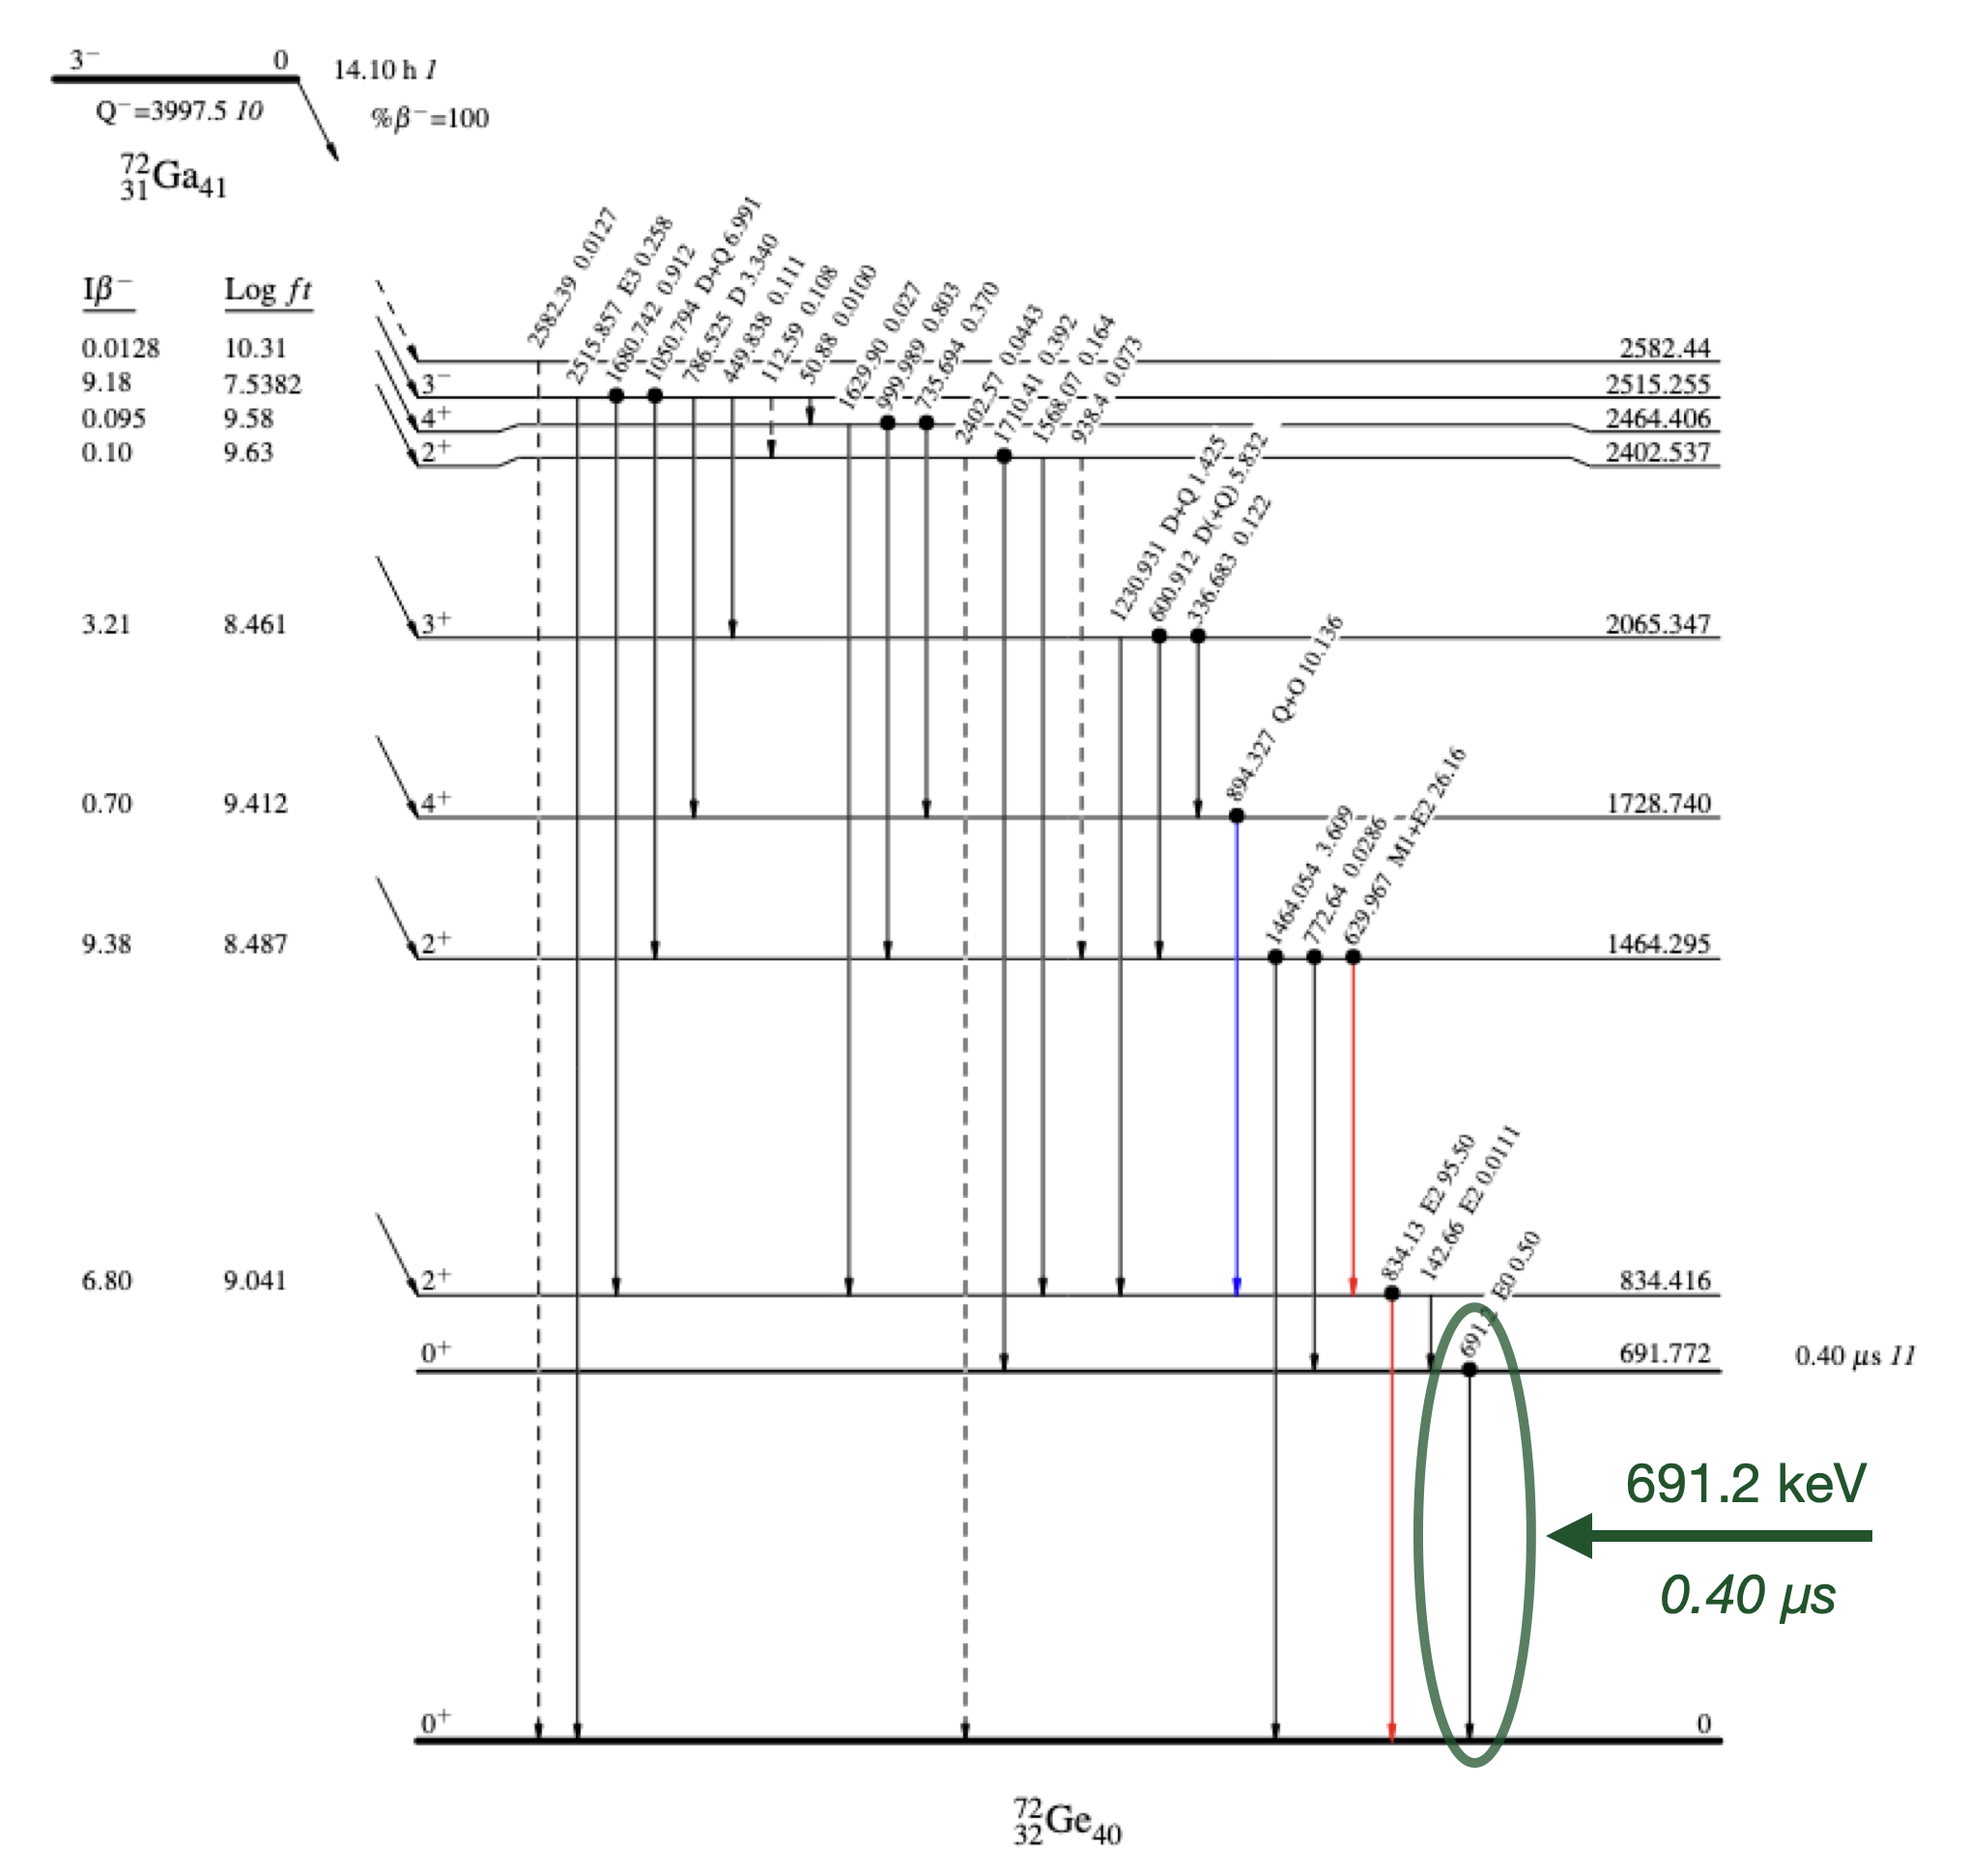
\includegraphics[width=0.95\textwidth]{ga72_beta_decay_level_scheme.png}
  \caption{Partial level scheme of $^{72}$Ge from the $\beta$ decay of $^{72}$Ge with the possible two-photon level indicated in green. Image from ENDSF.}
  \label{fig:ga72_level_scheme}
\end{figure}

%------------------------------------------
\subsection{Previous Work}
%------------------------------------------
The dataset for $^{72}$Ge has already been analyzed in detail for angular correlations and internal conversion coefficients. 
To look at angular correlations the data had to be conditioned with a robust energy calibration, cross-talk corrections applied, and detector efficiencies determined.
\ref{fig:efficiency_carlotta} shows the absolute efficiency curves for both the 2017 and 2019 datasets.
The angular correlation for the $2_2^+ \rightarrow 2_1^+ \rightarrow 0_1^+$ 630-834 keV $\gamma$-ray cascade in $^{72}$Ge was extracted and is shown in~\ref{fig:angular_correlation_carlotta}.
A more in depth discussion of what has been measured is given in~\cite{porzio_configuration_2021}, but the most crucial element of the previous analysis is the energy-calibration and data conditioning applied providing a simple route to extend the analysis to include a search for two-photon decay. 

\begin{figure}[htbp]
  \centering
  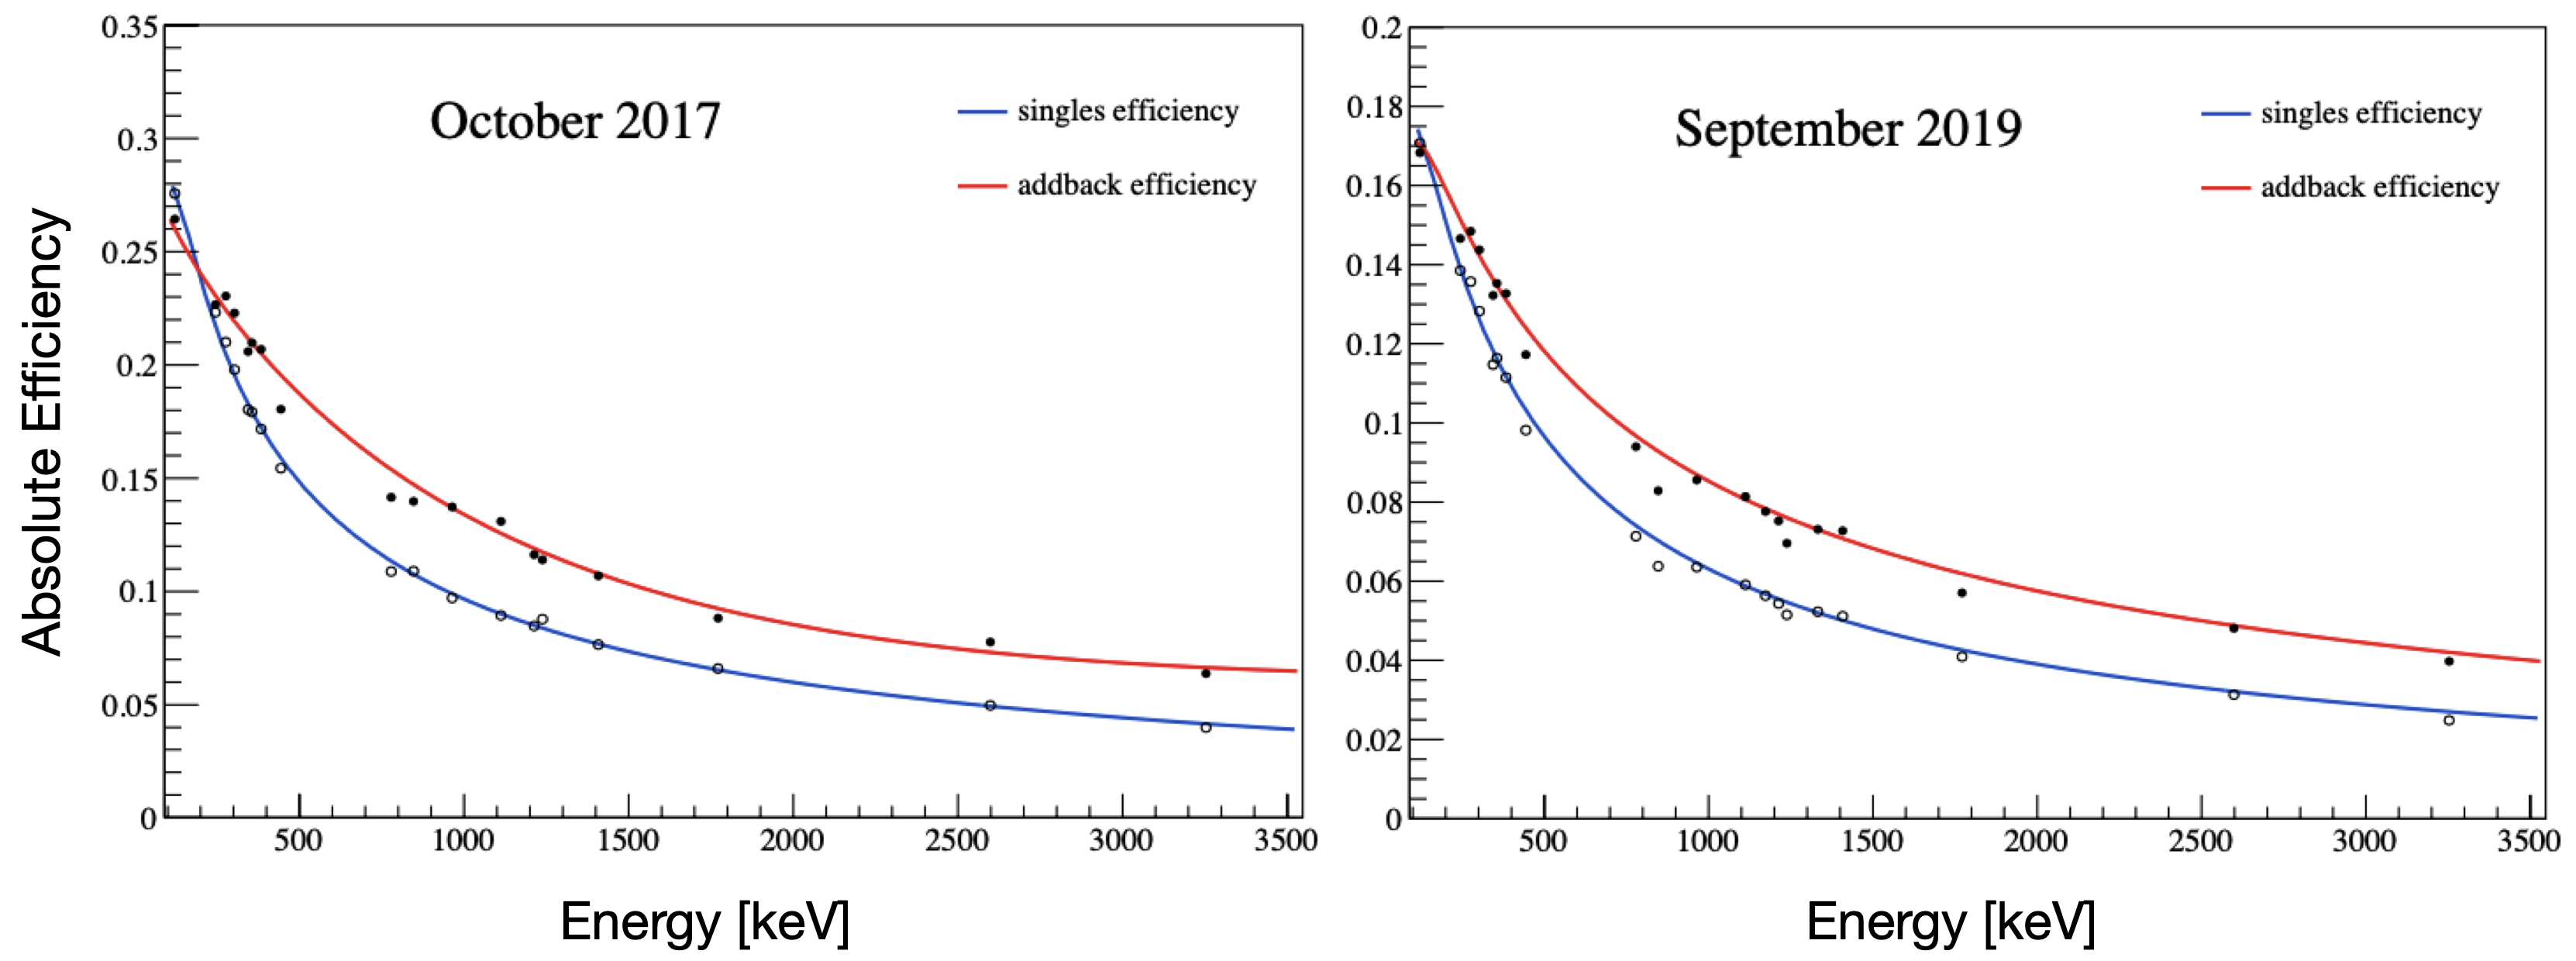
\includegraphics[width=0.95\textwidth]{efficiency_carlotta.png}
  \caption{Efficiency curves for GRIFFIN obtained with $^{152}$Eu, $^{56}$Co, $^{133}$Ba, and $^{60}$Co. Error bars are not visible because they are smaller than the marker size. Figures from~\cite{porzio_configuration_2021}.}
  \label{fig:efficiency_carlotta}
\end{figure}

\begin{figure}[htbp]
  \centering
  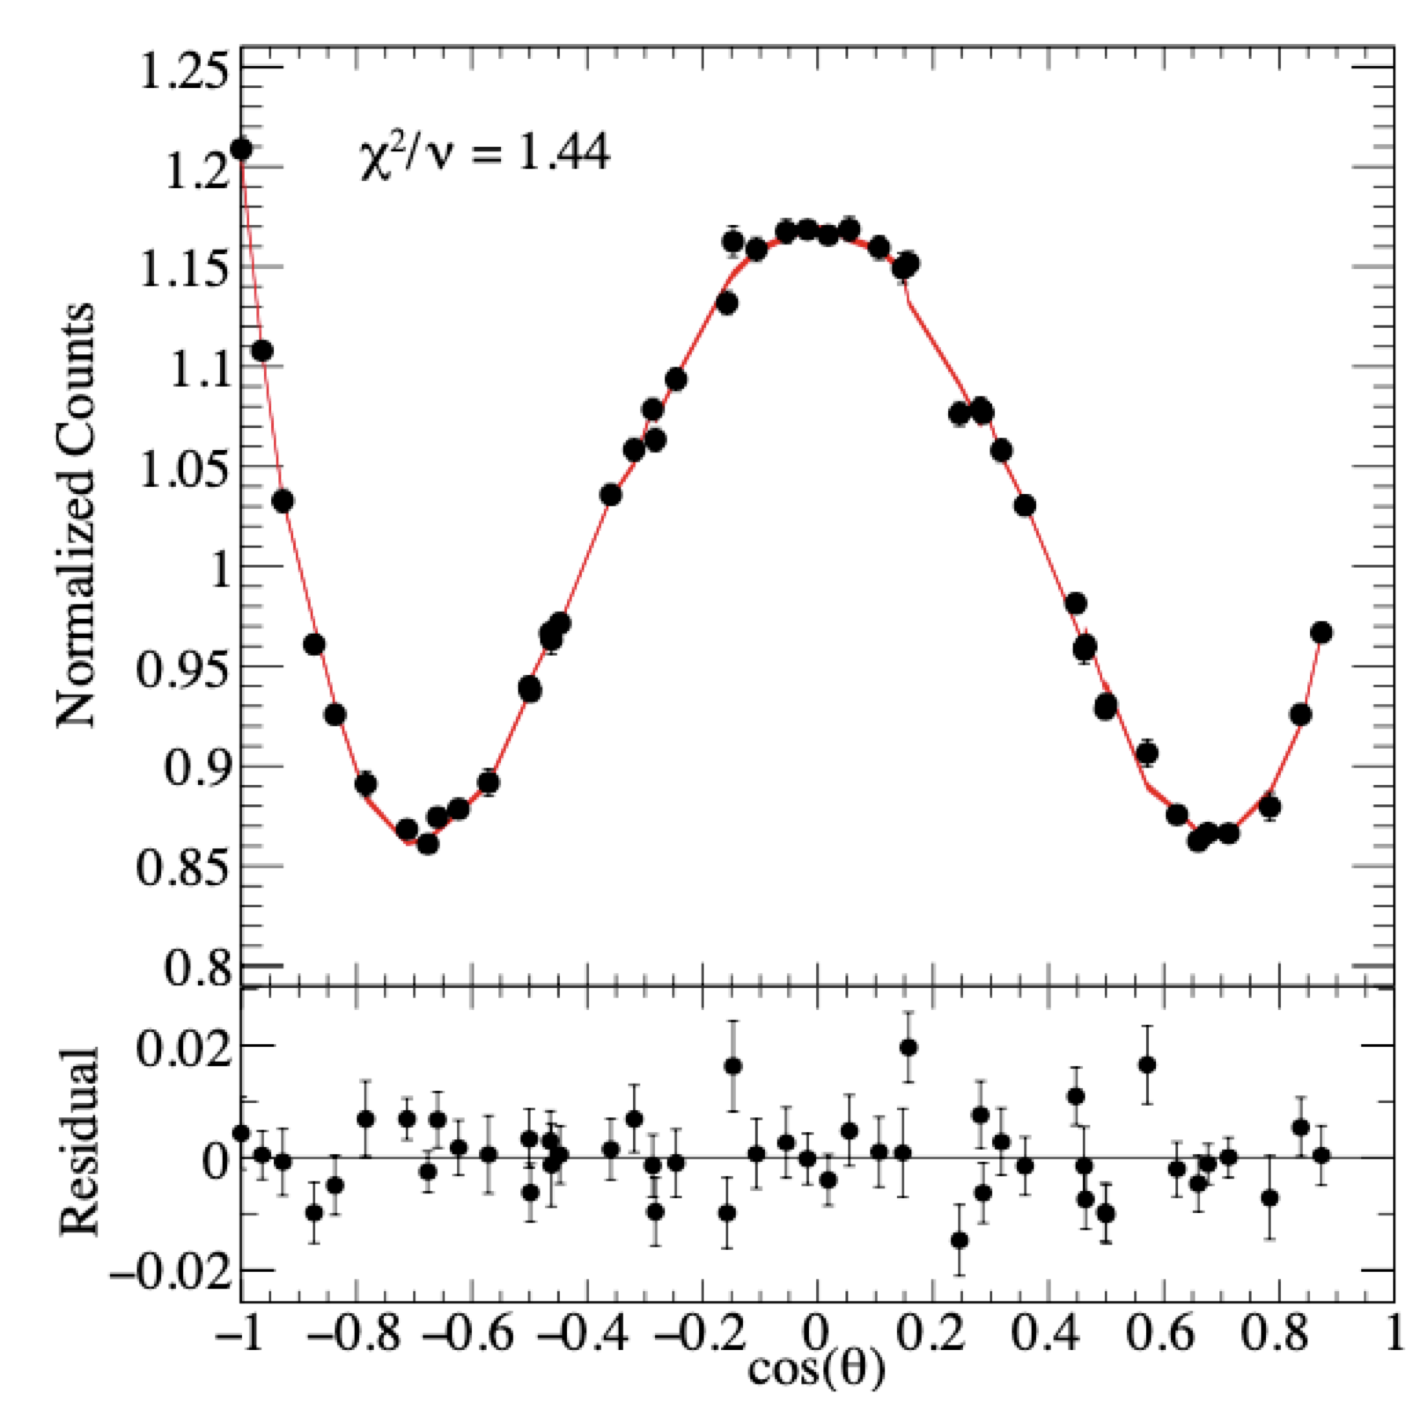
\includegraphics[width=0.95\textwidth]{angular_correlation_carlotta.png}
  \caption{Experimental angular correlation from the $2_2^+ \rightarrow 2_1^+ \rightarrow 0_1^+$ 630-834 keV $\gamma$-ray cascade in $^{72}$Ge extracted by C. Porzio. Figure from~\cite{porzio_configuration_2021}.}
  \label{fig:angular_correlation_carlotta}
\end{figure}


%------------------------------------------
\subsection{Extension of Analysis for Two-Photon Decay}
%------------------------------------------
As discussed in the previous sections the data already exists for the $\beta$ decay of $^{72}$Ga into $^{72}$Ge and the data has been conditioned such that calibrations and corrections are not necessary to extend the analysis. 
Proper coincidence timing gates must be determined to properly exclude the prompt decays from higher laying states in $^{72}$Ge and isolate the $\gamma$-rays from the 400 ns lifetime first excited state. 
Once the proper events are selected, a three-fold coincidence algorithm can be applied to extract possible two-photon events. 
The selected events must satisfy the following: 

\begin{itemize}
  \item The two $\gamma$-rays must be coincident within 30 ns of each other.
  \item A beta particle must be coincident within 20-50 ns of the two gammas respectively.
  \item The two $\gamma$-rays must sum to the full transition energy of 691.2 keV
\end{itemize}

Once the two-photon events are identified an energy sharing distribution can be identified given a sufficiently large number of statistics. 
Regardless of whether an energy distribution can be extracted identification of two-photon decay in $^{72}$Ge would be the first observed two-photon decay in that isotope and the fourth overall. 


%------------------------------------------
\end{document}
%------------------------------------------
